\documentclass[11pt]{article}
\usepackage{cs65f12}
\usepackage{times}
\usepackage{latexsym}
\usepackage{ulem}
\usepackage{graphicx}
\usepackage{listings}
\usepackage{color}
\usepackage[toc,page]{appendix}

\definecolor{dkgreen}{rgb}{0,0.6,0}
\definecolor{gray}{rgb}{0.5,0.5,0.5}
\definecolor{mauve}{rgb}{0.58,0,0.82}

\lstset{frame=tb,
  language=Java,
  aboveskip=3mm,
  belowskip=3mm,
  showstringspaces=false,
  columns=flexible,
  basicstyle={\small\ttfamily},
  numbers=none,
  numberstyle=\tiny\color{gray},
  keywordstyle=\color{blue},
  commentstyle=\color{dkgreen},
  stringstyle=\color{mauve},
  breaklines=true,
  breakatwhitespace=true
  tabsize=3
}
\setlength\titlebox{6.5cm}    % Expanding the titlebox

\title{BatTrace: Android battery performance testing via system call tracing}

\author{Yeayeun Park\\
{\tt ypark2@swarthmore.edu}
\And 
Mark Serrano\\
{\tt mserran2@swarthmore.edu}
\AND
Craig Pentrack\\                 
{\tt cpentra1@swarthmore.edu}}

\date{12/06/13}

\begin{document}
\maketitle
\begin{abstract}
  The increasing number of tasks we can perform on our mobile devices 
  feeds positively into the demand for devices with longer battery power. 
  Since mobile devices have become integral parts of our daily lives with
  the number of tasks we can accomplish far outpacing battery performance 
  improvements, consumers have increasingly encountered the issue of 
  efficient device usage and battery life management. In this paper, we 
  examine Android devices in particular and present BatTrace, an Android 
  analysis tool that evaluates battery performance on the android platform
  by tracing system calls. BatTrace will execute different types of popular system
  calls, and extract the correlation between a particular system call and its 
  influence on the battery. Subsequently, it will trace system calls made by 
  individual Android applications and use system call performance data to profile
  each application. Finally, the analysis on the correlation between system calls and their 
  battery usage, as well as the correlation between each application and system 
  calls they initiate, will be combined to estimate battery usage 
  of individual Android applications.
\end{abstract}

\section{Introduction}
Our project is motivated by an issue that we face daily: limited battery power 
on our mobile devices. The vast power available at our fingertips in mobile
devices is tamed by the amount of battery physically available. Wanting to track application behavior 
and the resultant energy usage, we used \textit{strace} in combination with C programs and Android system data to perform 
dynamic analysis on Android devices, uncovering low-level explanations as to what is really 
draining the battery.

Hypothesizing system calls to be the key to understanding battery usage at a low-level, we 
used \textit{strace} to profile applications system call usage.  Such testing gave us aggregate
statistics on which system calls were used and how often.  In the process of tracing popular
3rd party applications (e.g. Facebook, Gmail, etc.), we also recorded battery usage by utilizing
built in Android system data pre and post traces.  

Once aware of the most used system calls, we created C programs to repeatedly run those calls and
collect battery statistics.  It is important to note that in future versions of BatTrace we will need to collect
statistics on all system calls, as the most frequent calls may not drain the most power.  However, starting with the 
most frequent system calls and the C programs repeatedly ran, we acquired an avetage measure of how much battery each system call 
consumes.  From the aggregate trace data and average system call consumption data, we were 
able to make predictions on battery usage of 3rd party applications.  In collecting high level 
data on battery consumption, we hope to better inform Android users which applications drain their 
battery level most, providing a good set of guidelines for mobile users to follow when low battery 
crisises hit.  With our fine-grained system call data, we hope to better inform software developers 
and hardware manufacturers which system calls consume the most power.   

\section{Background and related work}

Historically much power consumption research has focused on using utilization-based
methods (on individual components, e.g. CPU).  However, modern smartphones employ complex 
power strategies in device drivers and OS-level power management, sometimes rendering utilization as a poor 
model for representing power states and deducing battery usage ~\cite{pathak-systemcall}.  While 
sometimes strong correlation exists between utilization and power consumption, often 
applications have constant power consumption while in certain states (while 
utilization fluctuates) or have high power consumption while low utilization ~\cite{pathak-systemcall,google-androiddev}.  
Merely focusing on CPU and other component-specific 
utilization levels do not capture tail-power states and the more intricate workings of power management.
Additionally, measuring utilization via performance counters results in accuracy 
loss ~\cite{pathak-systemcall}.  

Instead of modeling power with utilization, system calls, the only way of 
interacting with hardware and performing I/O, serve as a much more precise indicator 
of power consumption ~\cite{pathak-systemcall}.  System calls, an indispensible aspect of mobile applications, 
provide accessible insight in how an application is using the underlying hardware.  Past work and tools, most 
notably eProf, show correlating application behavior with power usage (via system calls and power readings) has 
been more successful than utilization-based approaches ~\cite{pathak-systemcall,yoon-appscope,pathak-eprof,ding-signals}.  
Using the findings of eProf and other studies as justification, we measured and classified system 
calls on Android smartphones in terms of their effect on battery life.

While eProf foregrounded system calls as an effective indicator of changes in power
state, eProf used system calls as a means toward profiling applications' power 
consumption on a sub-routine level ~\cite{pathak-systemcall,pathak-eprof}.  Developing models based off of system 
calls supplied a powerful tool, however the eProf research did not study battery drain 
as a result of  particular system calls themselves and the frequency with which 
applications rely on certain system calls.  Other work in smartphone battery 
research, including detecting energy-related bugs, correlating wireless signal strength 
with battery consumption, and generating battery usage information on the process or 
application level, has relied on system calls ~\cite{yoon-appscope,pathak-bugs,ding-signals}.  We plan to supplement the 
research area by focusing our study on the system calls themselves, rather than using 
them as a means in tracking changes in power state, detecting bugs, measuring signal 
strength effects, or producing higher-level profilings as explored previously.

\section{Our Idea}

While dynamic analysis on traditional devices involves the most efficient use of finite 
computing resources, mobile devices introduce a new problem; finite power. The issue we 
immediately encounter when trying to analyze mobile software applications is that we 
\sout{almost} never have access to the source code of the applications. This is 
especially true given the fact that most mobile software is proprietary in nature, 
leaving open source software to the relics that are desktop computers.

\begin{figure}[h]
  \centerline{
        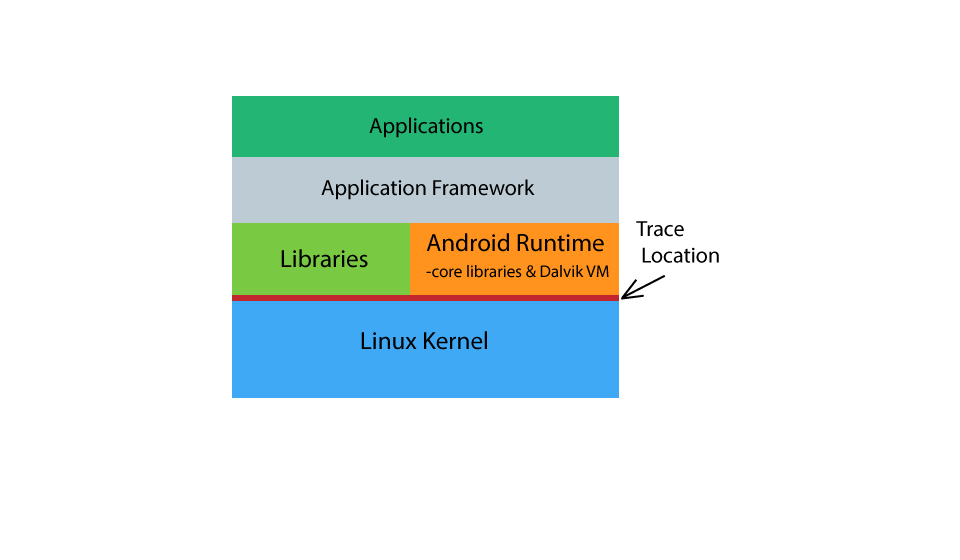
\includegraphics[width=90mm]{images/environment_graphic.png}
  }
  \caption{The Android environment stack. Trace location marks where we will be intercepting system calls}
  
 \end{figure}

With this in mind we set out find a way of measuring mobile battery usage at very low level
(software wise). We decided a good approach would involve monitoring activity at the system 
call level using \textit{strace}. We wanted to profile a variety of system calls 
based on how much battery is used while they are running. We intended to establish a baseline 
battery consumption level so we know how much battery is used by just the OS. Then, using 
simple programs that repeatedly make the same system call many times, as a single call is often
immeasurable, we can determine how much battery was used as a result of initiating a particular system call.  

Once system calls were profiled, we proceeded to the last phase of the analysis. Our 
goal was to identify the system calls initiated by the Dalvik VM as a result of running an 
individual app. By identifying the types of system calls, as well as the number of calls made 
to an individual system call, we were able to predict applications' impact on the battery based 
on what we learned about battery usage for individual system calls. While this approach may not 
be the most accurate, we believe it is an approach that will allow us to profile any 
application regardless of the author or the nature of the software's license.  While this design is 
not the only approach, with alternatives such as dynamic binary instrumentation, we think our way 
capturing system calls supplies the necessary information to properly model power usage by individual
Android applications.


\section{Evaluation}

In the process of analyzing battery usage through system call tracing we successfully
found most used system calls by popular Android applications, wrote C programs to 
repeatedly execute those system calls, recorded battery usage as a result of particular 
system calls, gathered system call data of popular apps dynamically, and made predictions 
based on the aforementioned data.  This section is split into subsections based on the above
categories.

\subsection{Frequent System Calls}

In relating system calls to battery usage, we first traced 10 popular Android
applications to acquire a list of the most frequent system calls.  We traced Google Maps, 
Facebook, Angry Birds, Youtube, Google Play, Gmail, Twitter, Skype, Pandora, and Instagram 
using \textit{strace}, collecting the ten most used system calls by each.  Applications were 
run for at least 2 minutes simulating normal usage patters.  More detailed information on the usage 
patterns appears in the Appendix with the system call frequency results appearing in the Table 4.1.1.

We found there were 14 most frequent, unique system calls among the applications tested.  Some of the 
systems calls in the 14 did not make the top ten as often (and munmap never), however these calls if 
not in the top ten often fell just outside it, so we decided to include them.  With this list, we knew 
some significant system calls to recreate in order to gather battery usage data.  A complete test 
should include all of the systems calls run, however we focused on the most frequent calls in 
this early stage of our research.  Later, including all system calls will be important as the frequent 
calls are not necessarily the system calls responsible for using the most power. 
\newline
\begin{tabular}{l c}
   System Call & \# Appearances \\
   \hline
   clock\_gettime & 10 \\
   ioctl & 10 \\
   getpid & 10 \\
   epoll\_wait & 10 \\
   getuid32 & 10 \\
   futex & 10 \\
   mprotect & 10 \\
   cacheflush & 9 \\
   read & 7 \\
   write & 6 \\
   sigprocmask & 4 \\
   gettid & 2 \\
   gettimeofday & 1 \\
   mmap2 & 1 \\
   munmap & 0 \\ 
\end{tabular}
\newline
{\fontsize{11}{13}\selectfont Table 4.1.1 Frequent System Calls in Popular Android Applications. Appearances denote how many
times a certain system call was in a top 10 most frequent system call list for each of 10 different applications tested.}
\newline

\subsection{System Call C programs}

In developing averages for battery usage per system call, we created C programs for each of the 14 unique system 
calls.  Once these programs were created, we ran a bash script running directly on the device that took a battery 
reading before and after each program completed.  An example system call C program can be seen in the Appendix.  

While the execution time and number of calls made varied among programs, they all ran for at least ten minutes, giving
us a significant change in battery. After running the script for each program, we recorded an average of battery level 
consumption per system call for each of the 14 unique most frequent.  See results in Table 4.2.1.

\begin{tabular}{l c}
   System Call & \# Battery Consumption \\
   \hline
   clock\_gettime & 0.006425 \\
   ioctl & 0.011998 \\
   getpid & 0.004161 \\
   epoll\_wait & 0.009926 \\      
   getuid32 & 0.006628 \\
   futex & 0.005474 \\
   mprotect & 0.006501 \\
   cacheflush & 0.004312 \\
   read & 0.010881 \\         
   write &  0.016212 \\        
   sigprocmask & 0.005274 \\
   gettid & 0.003000 \\
   gettimeofday & 0.008013 \\
   mmap2 & 0.006066 \\
   munmap &  0.006474\\              
\end{tabular}
\newline
{\fontsize{11}{13}\selectfont Table 4.2.1 Battery Consumption of System Calls. For readability consumption is displayed
per every 1,000,000 calls.}
\newline

Even at the level of a million calls, the battery consumption average for each system call was very small.  Such small battery drain of 
most calls made us critical of our experimental design, measuring the average drain of a particular system call by repeatedly running it.  
Futhermore, each unique system call was rerun using the same parameters, while the parameters of system calls made by 3rd party 
applications varied.  In the future, we plan to capture the battery drain of system calls in the wild, considering parameters.  A more detailed 
discussion of how we modeled power and future improvements continues in the analysis of error and future work section.  While being wary 
of our battery consumption averages for the 14 system calls tested, realizing our method of modeling power needs revision, we continued with our predictions.

\subsection{Prediction Data}

To make our predictions on battery usage of popular Android applications based off of battery consumption per call statistics,
we needed a complete list of system calls made by those applications, in particular at this stage getting the number of times 
each system call was made.  Using \textit{strace}, we attached to application-specific processes and recorded the necessary data. 
Before and after attaching to processes, we recorded the battery level of the Android device to enable later comparison between 
predicted consumptionand observed battery consumption.  The Android applications we used for predictions included Google Maps, 
Facebook, Youtube, and Pandora.  Observed consumption data can be found in Table 4.4.1.

\subsection{Predictions}

With prediction data (which systems calls are made by certain applications with their frequencies) and average consumption per
call for the 14 system calls we focused on, predicting battery usage was a matter of summing the estimated consumption for each 
system call.  We predicted each system call's power usage by multiplying the number of times it was called by our estimated 
usage for that particular call.  As we did not consider parameters at this stage in our research, the estimated battery usage for a 
call was the same for each call within an application and across applications.  We admit such oversimplication.  Once taking this sum, we added a baseline reading of how much power is used by tracing an almost completely idle application (we used weather clock) to simulate power used by the system, enabling accurate comparison to the traced 3rd party applications. 

When calculating these predictions, we only had the ability to include consumption of system calls for which we had average consumption statistics.  
While this is not complete and may seem limiting, the 14 unique calls we focused on were the top 14 used system calls for each application tested.  Comparison between predicted consumption and observed consumpted can be seen below in Table 4.4.1.

\begin{tabular}{l c r}
   Application & Predicted & Observed \\
   \hline
   Google Maps & 2 & 6 \\
   Facebook & 2 & 4 \\
   Youtube & 2 & 5 \\
   Pandora & 2 & 4 \\
\end{tabular}
\newline        
{\fontsize{11}{13}\selectfont Table 4.4.1 Battery Consumption Predictions and Observations.}
\newline

After seeing the differences between predicted and observed battery consumption for the applications tested, our suspicions surrounding 
the way we gathered average battery consumption per system call were made stronger. The predictions, due to the very small estimated 
drain of each system call, were equal to the baseline measure of tracing the mostly idle weather clock.  The predicted consumption 
as a result of system calls was insignificant.  We explore our sources of error and directions of future work in the next section, 
outlining how our predictions can be improved. 

\subsection{Analysis of Error \& Future Work}
Our project turned out to have had inherent flaws in the experimental design that naturally led to errors--the difference between the predicted 
values and the actual readings, as can be witnessed from the Table 4.4.1. We have identified three main issues that we discuss 
in this section:

\begin{itemize}
  \item Lack of system call parameters: Parameters are passed to system calls in the same way that they are passed to other functions. 
  These parameters contain important information that guides a system call’s behavior. Same system calls with different parameters are essentially 
  carrying out different tasks. In the C programs that we wrote (example shown in Appendix), we ran system calls with generic parameters that do not necessarily match those that were actually called in the test applications. In other words, it is possible and likely that system calls with varying parameters will drain battery differently. Thus, error existed in creating a average consumption for each call based on a single set of parameters while not considering the parameters of test applications.   
  \item Insufficient data collection: Our predictions are calculations of data from 14 most frequent system calls instead of all the system calls 
  initiated by the test applications. This design fails to capture the power consumption of less frequent system calls, and in particular less frequent system calls that use relatively high power. Due to this limitation, the power usage data we managed to collect from the top 14 system calls was not fully indicative of the actual power usage. 
  \item Design of our C programs: We designed our C programs so that each runs a single system call repeatedly in a for loop for a set number of iterations. Though this was a clever manipulation of the knowledge we were given, we concluded that it might not have been the best design. For instance, when ``getpid'' is called the first time, the value returned from calling the system call is almost certainly cached. Thus, for the rest of the iterations, power usage is significantly diminished, giving lower power usage than would occur in the wild where the sequence of system calls would differ. 

In the future, we would like to improve upon these errors, making our experimental design more accurate and complete. Furthermore, we hope to expand our project, so that it can be used as a useful guide for battery-conscious smartphone users.  In particular, we hope to make an downloadable tool that provides online analysis.
\end{itemize}

\section{Conclusions}

Despite the success of system call tracking on the mobile device, it is clear system calls alone do not provide an absolute measure of power consumption.  Though
we discuss some of the possible reasons why the predictions of our model were so far off, it is unlikely that these reasons are solely responsible for the
differences between the predicted values and the actual battery readings.  During our testing, it became apparent to us that additional power drain was
occurring as a result of higher level processes that did not interact directly with the underlying OS.  We suspect the Dalvik VM and the Java code being
executed on contributed to the power drain observed.  However, while system calls do not reliable provide an absolute measure, they proved to be useful in
calculating a relative measure of power efficiency across applications.  By running a variety of apps for a set amount of time, we were able to measure
power consumption via the system calls they triggered and, in turn, use the power consumption data to compare the applications to each other.  A tool such as
the one proposed in this paper could one day be part of the off-line development suites of software writers across the globe as the focus on energy efficiency shifts
from hardware to software.  However, this tool could also prove useful as an online in the hands of the consumer as consumers become more aware of power hungry applications and their effects on battery life.  While we were unable to develop a solid measure of battery drain using the proposed model, the approach still shows promise and our work provides a solid foundation on which to develop additional research.

\bibliographystyle{cs65f12}
\bibliography{cs65f12}

\newpage
\appendix
\section{\\Appendix} \label{App:AppendixA}

\subsection{Tasks Done When Tracing}

When we traced popular Android applications -- Google Maps, 
Facebook, Angry Birds, Youtube, Google Play, Gmail, Twitter, Skype, Pandora, and Instagram --
in determining which C programs to recreate and in collecting prediction data we tried our
best to simulate normal usage patterns.  When using Google Maps we asked for directions, explored
the map, went into street view, and looked for places to eat. For Facebook we browsed the Newsfeed, 
liked posts, wrote a new post, and looked at friends' pages.  Below is a list of the tasks performed 
for each of the test applications when getting the most frequent system calls. When getting prediction
data, the tasks were much the same however carried out over a longer period of time (at 10 minutes instead
of 2 minutes).

\begin{itemize}
  \item Google Maps: getting directions, moved around map zooming in and out, changing from the grid map
  to satellite imaging (street view), looked at location specific details 
  \item Facebook: browsed Newsfeed deep into endless scroll, interacted with posts in Newsfeed, authored
  new post, went to friends' profiles and interacted with them
  \item Angry Birds: completed the first 2 levels
  \item Youtube: searched for 2 videos playing segments of both, played segment of video from featured videos
  \item Google Play: browsed popular applications (free and paid), downloaded twitter
  \item Gmail: checked for new mail, composed new email, went into email history and read 
  \item Twitter: scrolled through personalized feed, searched for hashtags, clicked links to other users 
  \item Skype: entered into video chat, did some text chatting 
  \item Pandora: created new station, added variety to existing stations, listening to different stations
  throughout
  \item Instagram: scrolled through dash, looked through trending posts, liked several posts, looked at 
  user profiles
\end{itemize}

While simulating normal usage seemed important in capturing averages for system call battery drain and the most
frequent calls, future study should focus on usage patterns that generate a complete list of system calls with 
varying parameters.

\subsection{Example C Program}

When desigining tests to estimate the average consumption of the 14 unique system calls we considered,
we created C programs to repeatedly run the call, collecting battery data before and after via a bash script.
The basic structure of the C programs followed the example below.

\begin{lstlisting}
/* getclocktime.c */
#include <sys/syscall.h>
#include <time.h>
#include <stdlib.h>
#include <stdio.h>
#include <sys/types.h>
#include <unistd.h>
#include <sys/time.h>

int main() {
  struct timespec ts;
  unsigned long long i;

  //750,000,000 calls
  for(i=0; i<750000000; i++) {
    syscall(SYS_clock_gettime, CLOCK_REALTIME, &ts);
  }
  return EXIT_SUCCESS;
}
\end{lstlisting}

{\fontsize{11}{13}\selectfont Figure A.2.1 Example C Program for get\_clocktime system call.}
\newline

While this design will have to change in future work to improve predictions, we wanted to be as transparent as 
possible in how we acquired average battery consumption for each system call so far.

\end{document}
